\setlength{\parindent}{0pt}
\setlength{\parskip}{0.6em}

%----------------------------------------------------------------------------
\chapter{Preliminaries}
\label{chap:prerequisites}
%----------------------------------------------------------------------------

In this chapter, I will provide a brief introduction to the technologies that may not be considered common knowledge for computer engineers but are essential to understanding my thesis.

\section{Kubernetes}

This is how Kubernetes introduces itself on its website~\cite{K8s}: `Kubernetes, also known as K8s, is an open-source system for automating deployment, scaling, and management of containerized applications.'

It stands as one of the most popular platforms for operating large-scale distributed applications. In response to the growing complexity of modern applications, Kubernetes offers a robust and flexible solution to streamline the orchestration and management of containerized workloads.

A key strength of Kubernetes lies in its declarative approach to configuration. The desired state of the applications is defined using YAML manifests, specifying details such as container images, resource requirements, and scaling policies. Kubernetes then takes on the responsibility of ensuring that the current state matches the declared state, automatically managing container lifecycles, scaling, and load balancing.

However, given the inherent complexity of the problems Kubernetes addresses, implementing it correctly can be challenging. Suboptimal configurations are common, and my thesis project seeks to provide a solution for optimizing the operation of applications in Kubernetes.

\subsection{Admission controllers}
\label{sec:admcont}

TODO global add ~ before \textbackslash cite

The official documentation~\cite{K8sAdmissionOfficial} explains admission controllers as the following:

`An admission controller is a piece of code that intercepts requests to the Kubernetes API server prior to persistence of the object, but after the request is authenticated and authorized.'

A very informative blog~\cite{K8sAdmissionBlog} on the topic, which I recommend reading, summarizes them like this:

`In a nutshell, Kubernetes admission controllers are plugins that govern and enforce how the cluster is used. They can be thought of as a gatekeeper that intercept (authenticated) API requests and may change the request object or deny the request altogether.' 

For detailed information, I recommend reading the cited~\cite{K8sAdmissionBlog} source or referring to the official documentation~\cite{K8sAdmissionOfficial}.

\begin{figure}[h]
    \centering
    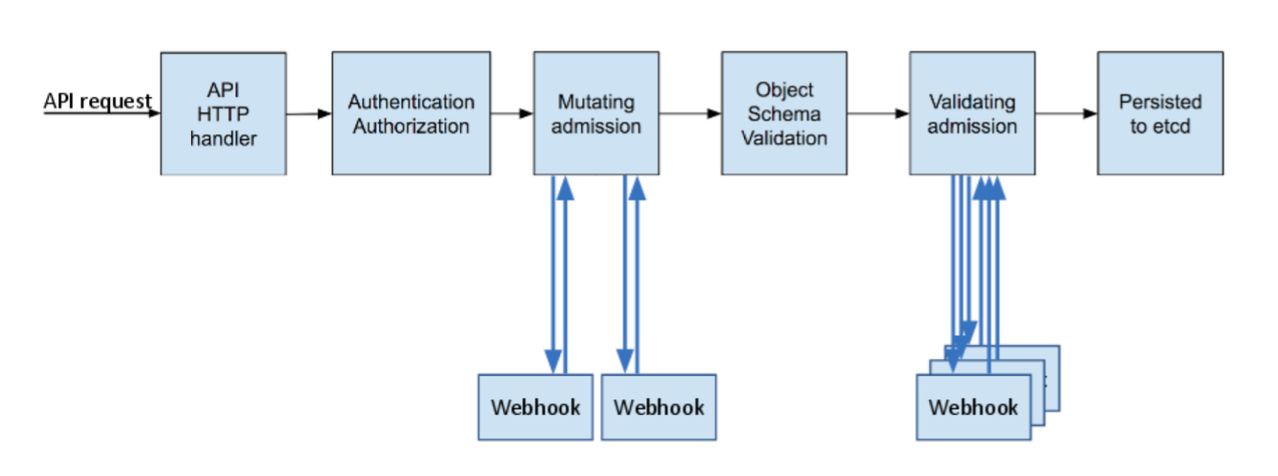
\includegraphics[width=130mm, keepaspectratio]{content/10_prerequisites/dynadm.png}
    \caption{Admission Controller Phases~\cite{K8sAdmissionBlog}}
    \label{fig:dynadm}
\end{figure}

In my thesis uses these 

\url{https://www.baeldung.com/java-kubernetes-admission-controller}
\url{https://kubernetes.io/docs/reference/access-authn-authz/extensible-admission-controllers/}



\section{Kotlin}

Kotlin is a multi paradigm modern JVM language, with full interoperability with Java, and many features that are not present in languages like Java. These features are used extensively in my DSL, and this chapter is meant to introduce them.

\subsection{Extension functions}
\label{sec:extension}

An extension function can add new functionality to an existing class without modifying it~\cite{KExt}. In Java, this can be implemented as shown in the \ref{code:prelimkext1} code snippet. Although Java lacks native support for extension methods, there is a workaround using public static utility functions. In contrast, Kotlin supports extension functions natively, as demonstrated in the \ref{code:prelimkext2} code snippet.

\begin{lstlisting}[caption={Extension functions in Java},language=Java11,label=code:prelimkext1]
public class MyClass {
  ...
}
public class MyClassExtensions {
  private MyClassExtensions() {}
  public static void myExtensionFunction(MyClass self) {
    self.doSomething();
  }
}
// Invocation:
final var myClass = new MyClass();
myExtensionFunction(myClass);
\end{lstlisting}

\begin{lstlisting}[caption={Extension functions in Kotlin},language=Kotlin,label=code:prelimkext2]
class MyClass {
  ...
}
fun MyClass.myExtensionFunction() {
  this.doSomething()
  // Using the "this" keyword is optional
}
// Invocation:
val myClass = MyClass()
myClass.myExtensionFunction()
\end{lstlisting}

\subsection{Receivers}

The term `receiver' is closely associated with extension functions, where it refers to the class to which the function is adding new functionality. When discussinglambdas, the block of the lambda might also have a receiver. In both cases, the receiver can be accessed with the `this' keyword, similar to the containing object reference. Implicit receivers also exist, where the `this' keyword is not used explicitly.

\subsection{Null safety}

Kotlin is a null-safe language, which means it has native support to address the challenges and errors associated with null or undefined values. The key concepts are:

\begin{itemize}
    \item \textbf{Nullable and non-nullable types (`String?' and `String'):} There are distinct types for values that can never be null and types for values that might be null during the program's execution. If a value is allowed to be null, its type is marked with a question mark (?).
    \item \textbf{Safe calls (?.):} Calling a function on a nullable type is not allowed with the dot (.) operator, as it might result in a null pointer exception Instead, the safe call operator (?.) shall be used. The safe call only invokes the function if it is not null; otherwise, the entire expression will return null.
    \item \textbf{Elvis operator (?:):} It is an infix operator that returns its left-hand side operand if it's not null; otherwise, it returns it's right-hand side operand.
\end{itemize}

Unfortunately, when calling libraries written in Java, the strict null-safety rules need to be relaxed, as Java does not ensure null safety. In such cases, it is the responsibility of the programmer to handle values as either nullable or null-safe. This presented a significant challenge during my work, requiring the development of strategies to manage unsafe calls in my DSL scripts.

For more information on the relation of Kotlin null-safety and Java interoperability, I recommend reading the official documentation on the topic: \url{https://kotlinlang.org/docs/java-interop.html\#null-safety-and-platform-types}
